\documentclass[a4paper]{article}
%for math
\usepackage{amsfonts}
\usepackage{amssymb}
\usepackage{mathrsfs}
\usepackage{amsmath}
%for images
\usepackage{graphicx}

%for title
\title{Cauchy-Crofton Formula}
\author{Caroline \textsc{Bouat}, Aadil \textsc{Khan}, Chris \textsc{Bishop}, Paul \textsc{Dubois}}
\date{8th June 2018}



\begin{document}
\maketitle



\section{Definitions}
\subsection{Rigid Motion}
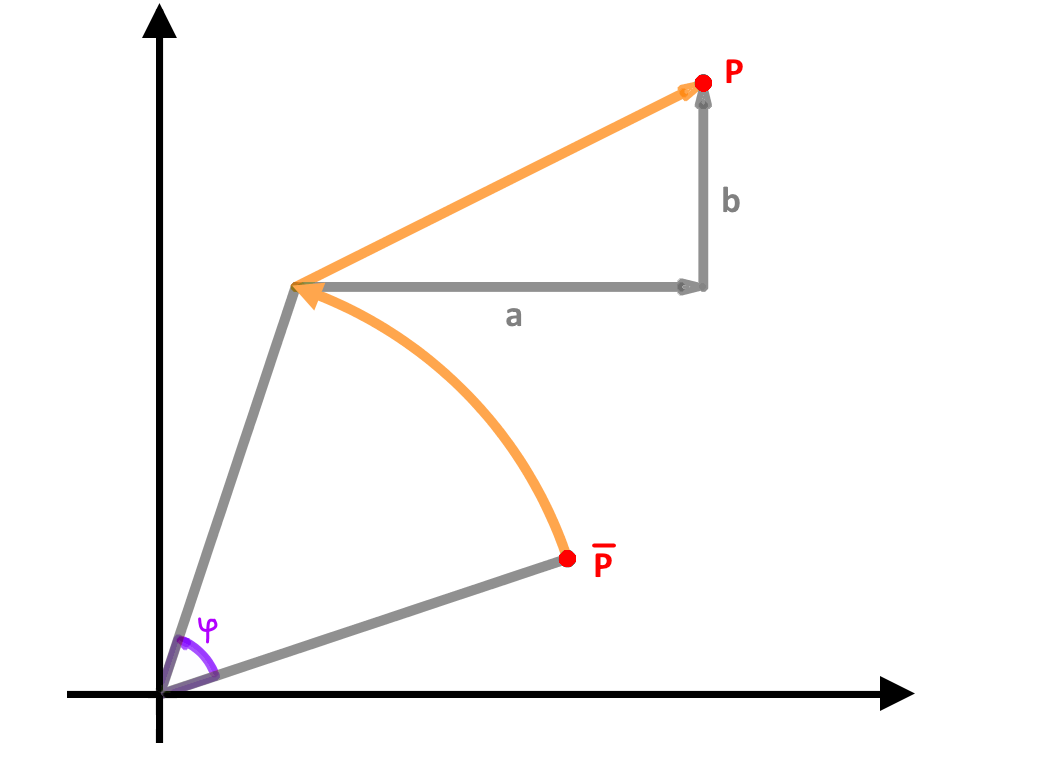
\includegraphics[width=360pt]{img/figureRigidMotion.png}
$$\overline{P} = (\overline{x}, \overline{y}) ; P = (x, y)$$
$$x=\overline{x} \cos (\varphi) - \overline{y} \sin (\varphi) + a$$
$$y=\overline{x} \sin (\varphi) + \overline{y} \cos (\varphi) + b$$
$$F:\mathbb{R}^2 \to  \mathbb{R}^2 \quad st \quad  F(\overline{P}) = P \quad \text{is a rigid motion}$$

\subsection{Measure}
%$F$ is called a delta-ring if $F$ is a ring and, for any countable collection of sets $\{A_n\}$ in $F$, the intersection intersection $A_n$ is also in $F$.
$F$ is a $\delta$-ring if:
\begin{itemize}
\item $F$ is a field
\item $\forall \{A_n \subset F \}_{n \in \mathbb{N}},  \quad \bigcap\limits_{n \in \mathbb{N}} A_n \subset F$
\end{itemize}

%A measure is defined as a non-negative real function from a $\delta$-ring $F$ such that:
If $F$ is a $\delta$-ring, a measure is a function $m: F \to \mathbb{R}^{+}$ such that:
\begin{itemize}
\item $m(\emptyset) = 0$
\item $A=\bigcup\limits_{n \in \mathbb{N}} A_n \subset F \implies m(A)=\sum\limits_{n \in \mathbb{N}} m(A_n)$
\end{itemize}

\subsection{Representation of lines in the plane}
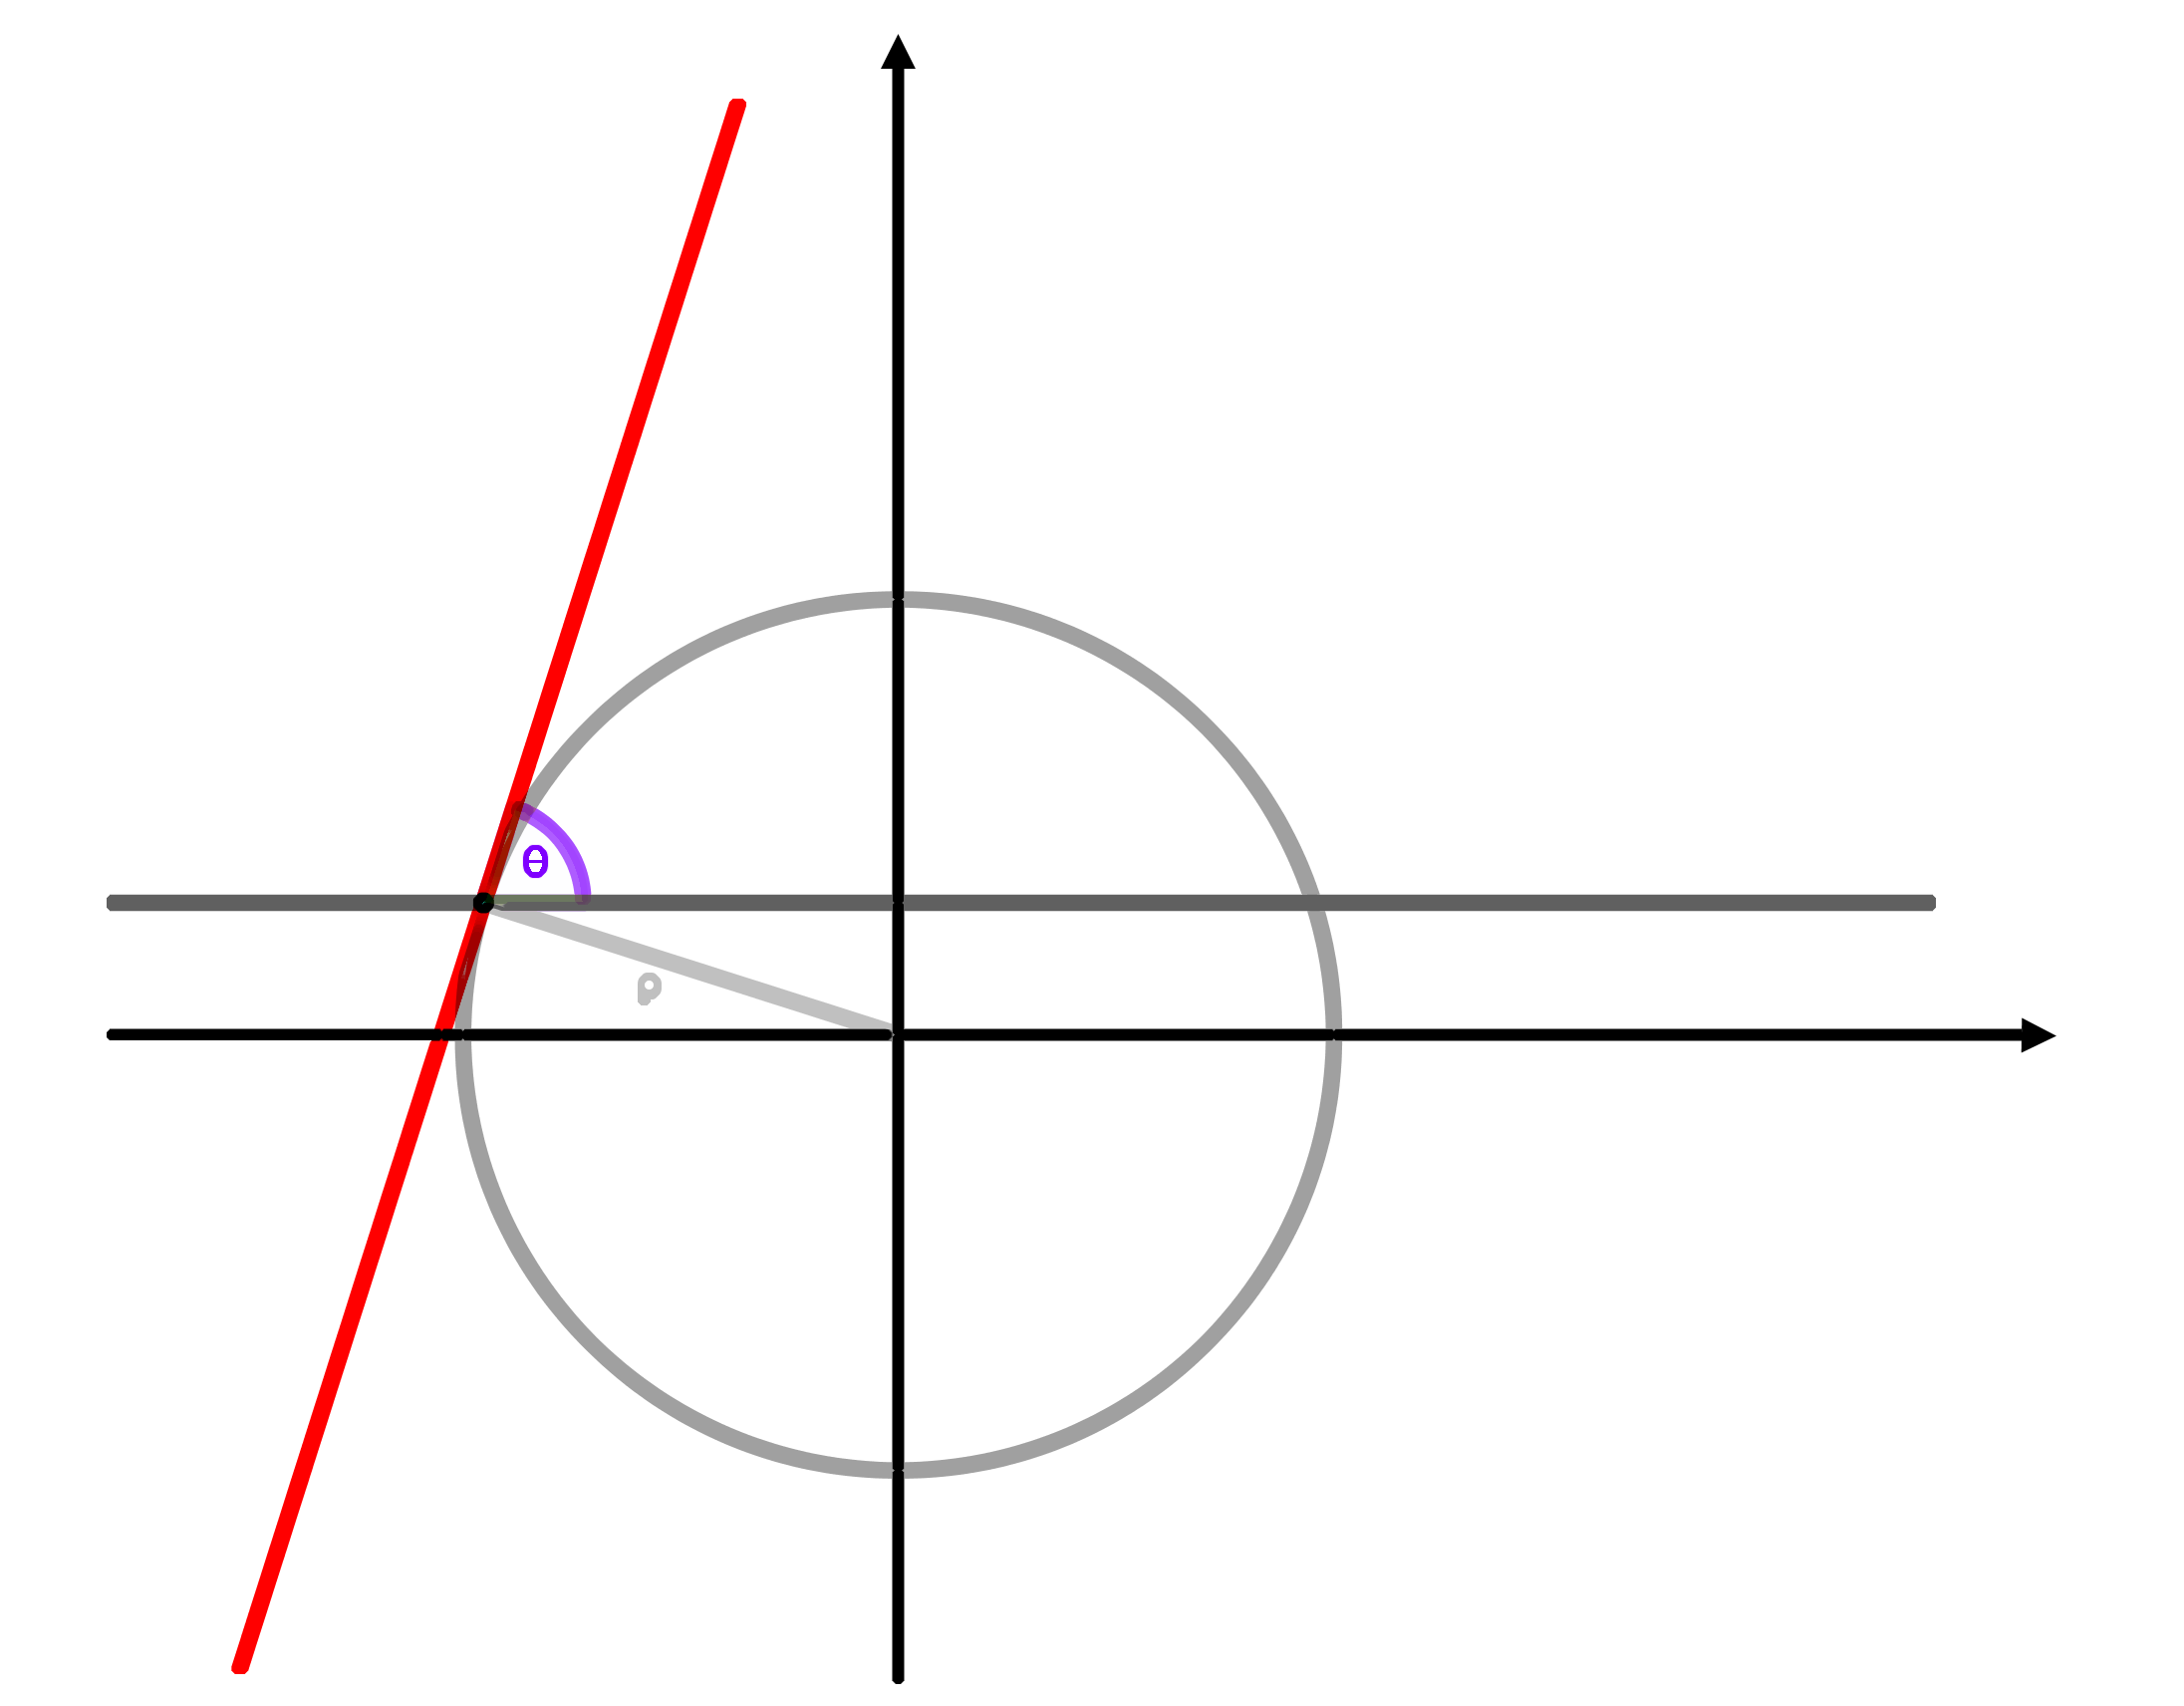
\includegraphics[width=360pt]{img/figureLineRepr.png}
Let $l$ be a straight line in the plane.
Then let $(\rho, \theta)$ be the representation by a point of the line $l$, where $\rho \geq 0$ is the distance of the line to the origin, and $\theta$ is the angle with the horizontal. So that 
$$l: x\cos(\theta) + y\sin(\theta) = \rho$$
Doing this, the set of all straight lines in the plane have representation 
$$\mathscr{L} = \{(\rho, \theta)  |  0 \leq \rho, 0 \leq \theta \leq 2\pi \}$$
Note that now the set of all lines in the plane are represented by a point in $\mathscr{L}$ which is a region in an other plane:

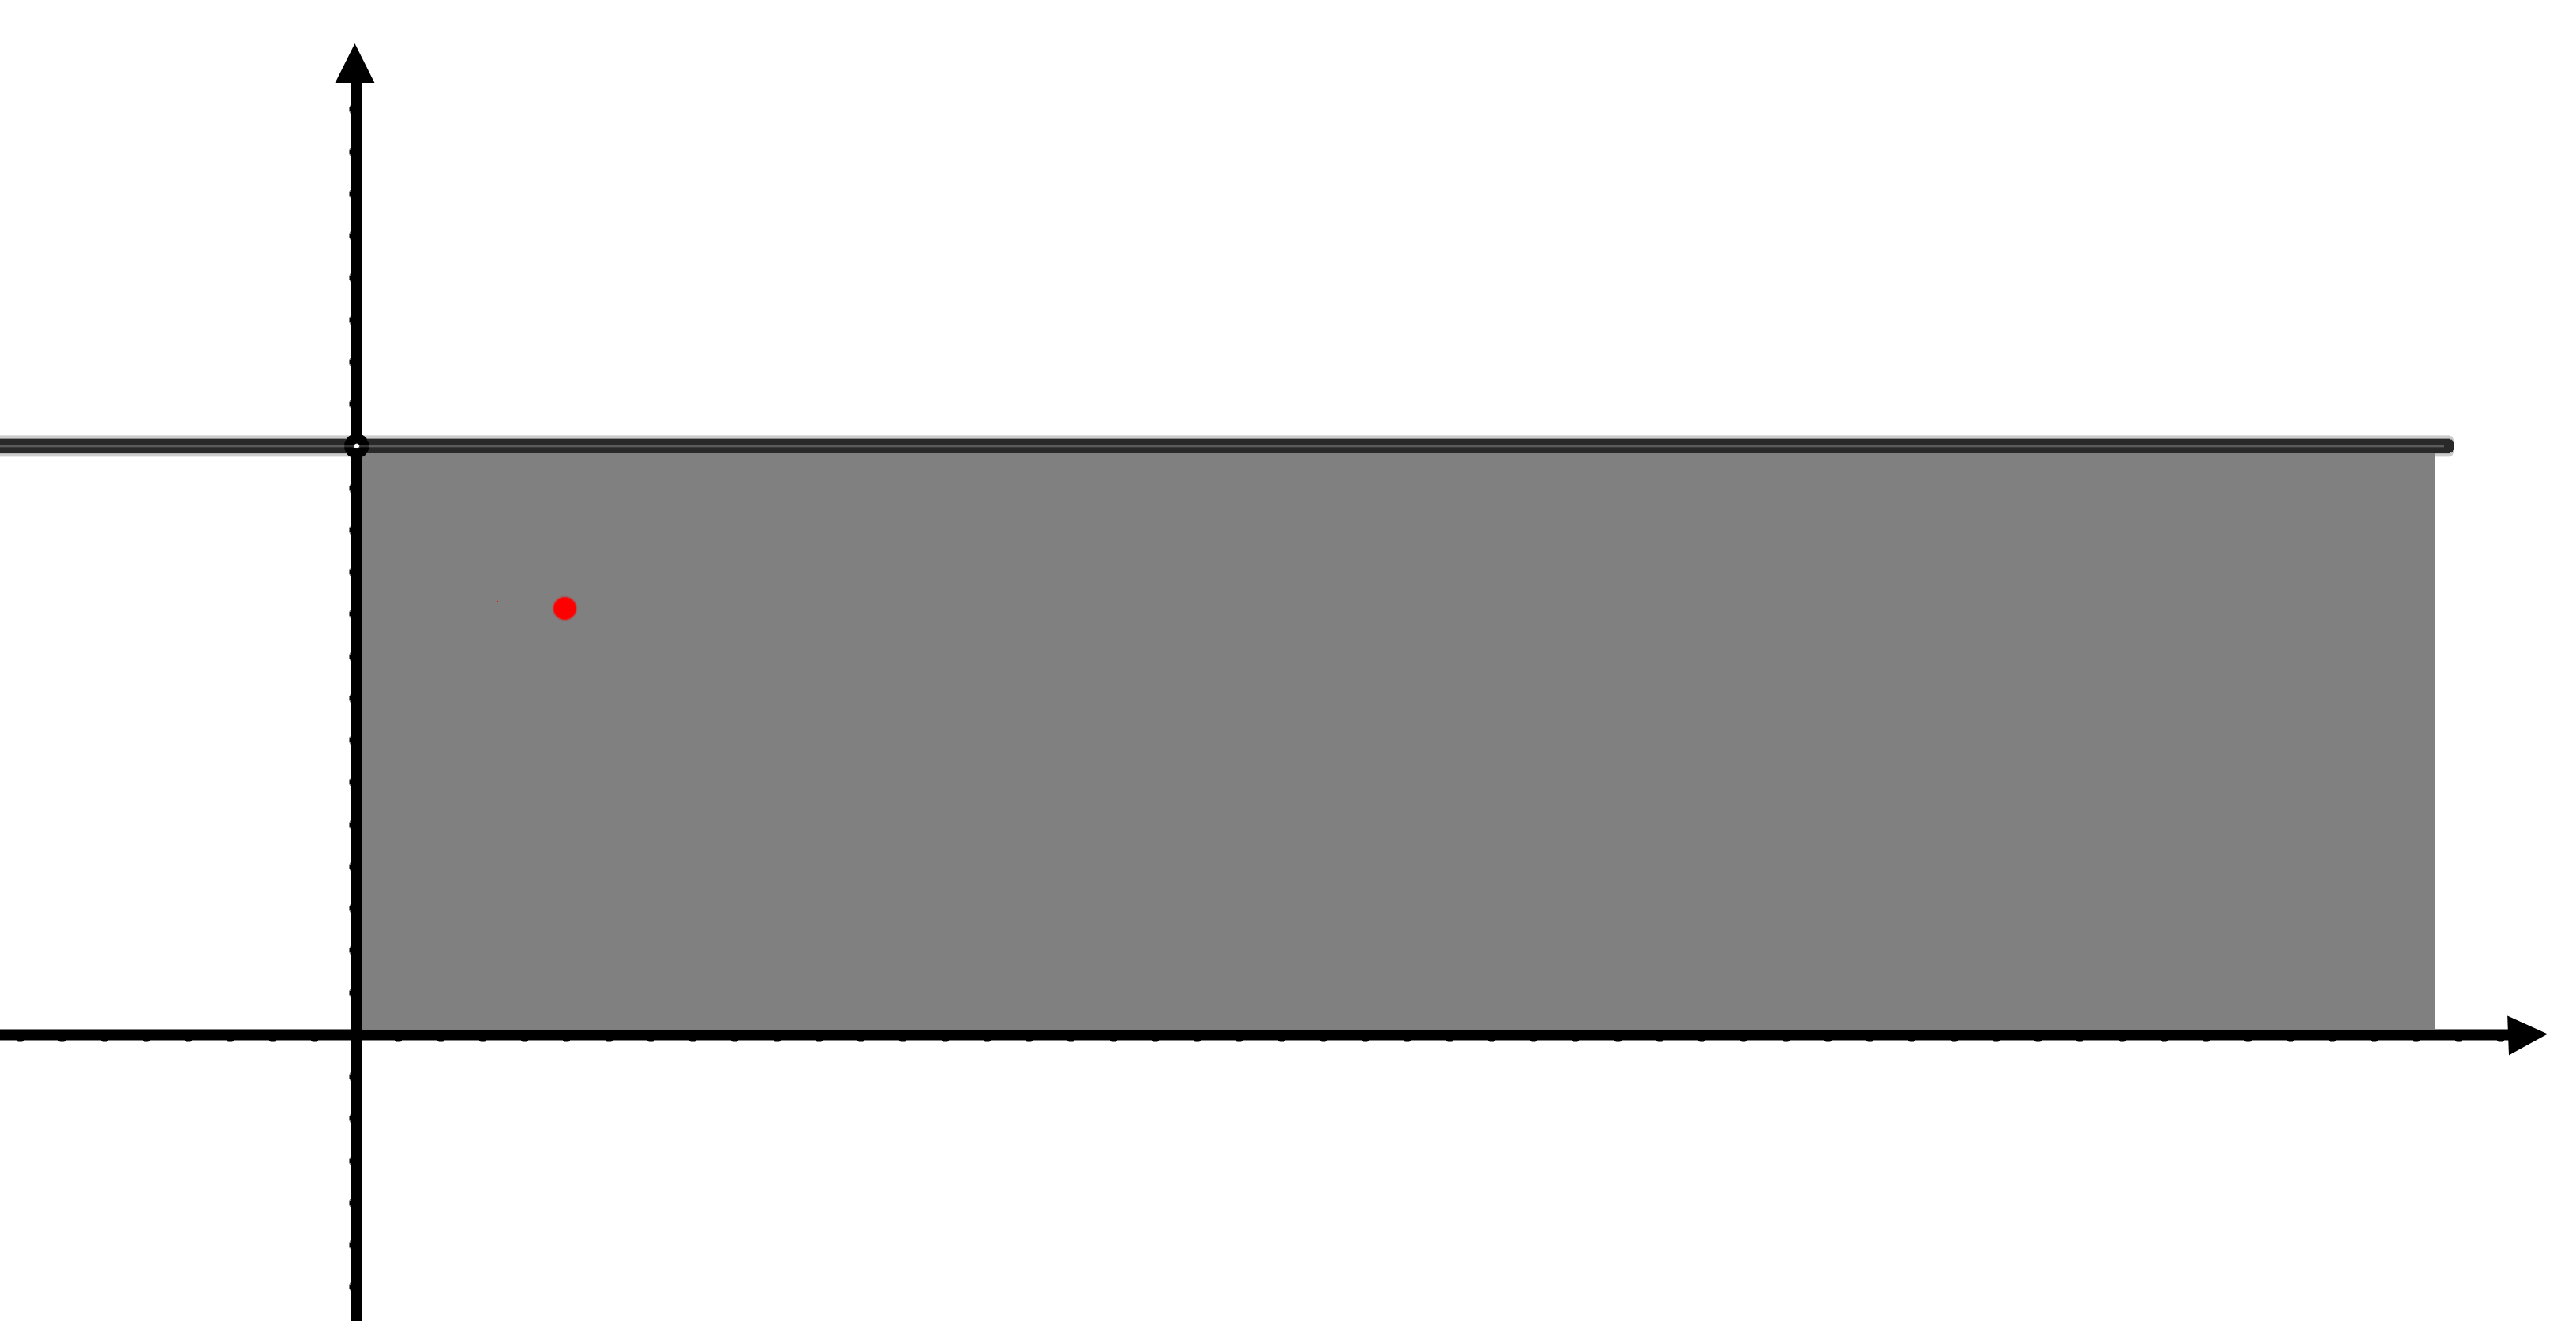
\includegraphics[width=360pt]{img/figureSetLines.png}




\section{Theorem}
Define a reasonable measure for the set of straight lines in the plane.
Let C be a regular curve in a plane. Then the measure of the set of straight lines that cross C (counted with multiplicity) is exactly twice the length of C.





\section{Proof}
\subsection{Reasonable measure is unique}
We want to define a measure on $\mathscr{L}$ such that the measure is independent of rigid motion. ("reasonable")
\smallbreak
As $\mathscr{L}$ is a portion of plane, to fit with the definition of a measure, we need our measure $m$ to be such that
$$m(S)=\iint_S f(u,v) \,du\,dv$$
%this a bit to clarify if we have time, later
with $f:\mathbb{R}^2 \to  \mathbb{R}^2$ continuous and $S$ the set of point that represent lines $l$ crossing a given curve C.
\bigbreak

Now, if we apply a rigid motion to the plane containing the curve, we get:
$$x=\overline{x} \cos (\varphi) - \overline{y} \sin (\varphi) + a$$
$$y=\overline{x} \sin (\varphi) + \overline{y} \cos (\varphi) + b$$
So the line $l$, represented by $(\rho, \theta)$ becomes:
$$x\cos(\theta) + y\sin(\theta) = \rho$$
$$\Leftrightarrow (\overline{x} \cos (\varphi) - \overline{y} \sin (\varphi) + a) \cos(\theta) + (\overline{x} \sin (\varphi) + \overline{y} \cos (\varphi) + b) \sin(\theta) = \rho$$
\begin{multline}
\Leftrightarrow \overline{x} \cos (\varphi) \cos(\theta) - \overline{y} \sin (\varphi) \cos(\theta) + \overline{x} \sin (\varphi) \sin(\theta) + \overline{y} \cos (\varphi) \sin(\theta) \\
= \rho - a \cos(\theta) - b \sin(\theta)$$
\end{multline}
$$\Leftrightarrow \overline{x} \cos (\varphi - \theta) + \overline{y} \sin (\varphi - \theta)  = \rho - a \cos(\theta) - b \sin(\theta)$$
which is a line (call it $\overline{l}$) represented by $(\overline{\rho}, \overline{\theta}) = (\rho - a \cos(\theta) - b \sin(\theta), \varphi - \theta)$
\bigbreak

$S$ is the set of lines that cross the curve C.
If $l \in S$, and $l$ is represented by $(\rho, \theta)$ then the line $\overline{l}$ represented by $(\overline{\rho}, \overline{\theta})$ will cross the curve C after applying rigid motion.
So, if $\overline{S}=\{(\overline{\rho}, \overline{\theta}) st (\rho, \theta) \in S \}$, then $\overline{S}$ is the set of point that represent the lines $\overline{l}$ with $l$ crossing C, so $\overline{S}$ is the set of points that represent lines that cross C after applying rigid motion.
\smallbreak
We want the measure to be independent of rigid motion, so:
\begin{align}
m(S) &= m(\overline{S}) \\
\Leftrightarrow \iint_S f(\rho,\theta) \,d\rho\,d\theta &= \iint_{\overline{S}} f(\overline{\rho},\overline{\theta}) \,d\overline{\rho}\,d\overline{\theta} \\
&= \iint_{\overline{S}} f(\rho (\overline{\rho},\overline{\theta}), \theta (\overline{\rho},\overline{\theta}))   \frac{ d\overline{\rho} \, d\overline{\theta} }{ d\rho \, d\theta }    \,d\rho \,d\theta \\
&= \iint_{\overline{S}} f(\rho, \theta) 
\begin{vmatrix} %matrices determinant
\frac{d\overline{\rho}}{d\rho} & \frac{d\overline{\rho}}{d\theta} \\ 
\frac{d\overline{\theta}}{d\rho} & \frac{d\overline{\theta}}{d\theta} \\ 
\end{vmatrix} 
\,d\rho \,d\theta \\
&= \iint_{\overline{S}} f(\rho, \theta) 
\begin{vmatrix} %matrices determinant
 1 & a\sin(\theta) - b\cos(\theta) \\ 
 0 &  1 \\ 
\end{vmatrix} 
\,d\rho \,d\theta \\
&= \iint_{\overline{S}} f(\rho, \theta) \,d\rho \,d\theta
\end{align}
As this should be true for all S and for all rigid motion, $f(\rho,\theta)$ can not depend on $\rho$ nor $\theta$. 
Therefore, $f(\rho,\theta)$ has to be constant. So up to a multiplicative constant, we have:
$$m(S)=\iint_S \,d\rho\,d\theta$$

\subsection{Particular case: a segment}
First, suppose that the curve is just a segment in the plane, and let $S$ be the set of straight lines that cross this segment.
If the curve is a straight line of length $l$, then we can apply a rigid motion to it so it becomes the segment on the $x$-axis that goes from $-\frac{l}{2}$ to $\frac{l}{2}$. The measure is invariant about rigid motion, so it remains the same after this operation.
Let $\theta$ be given, let's try to find a condition on $\rho$ for the line represented by $(\rho, \theta)$ to be crossing the segment we are considering (i.e. to be in the set $S$):

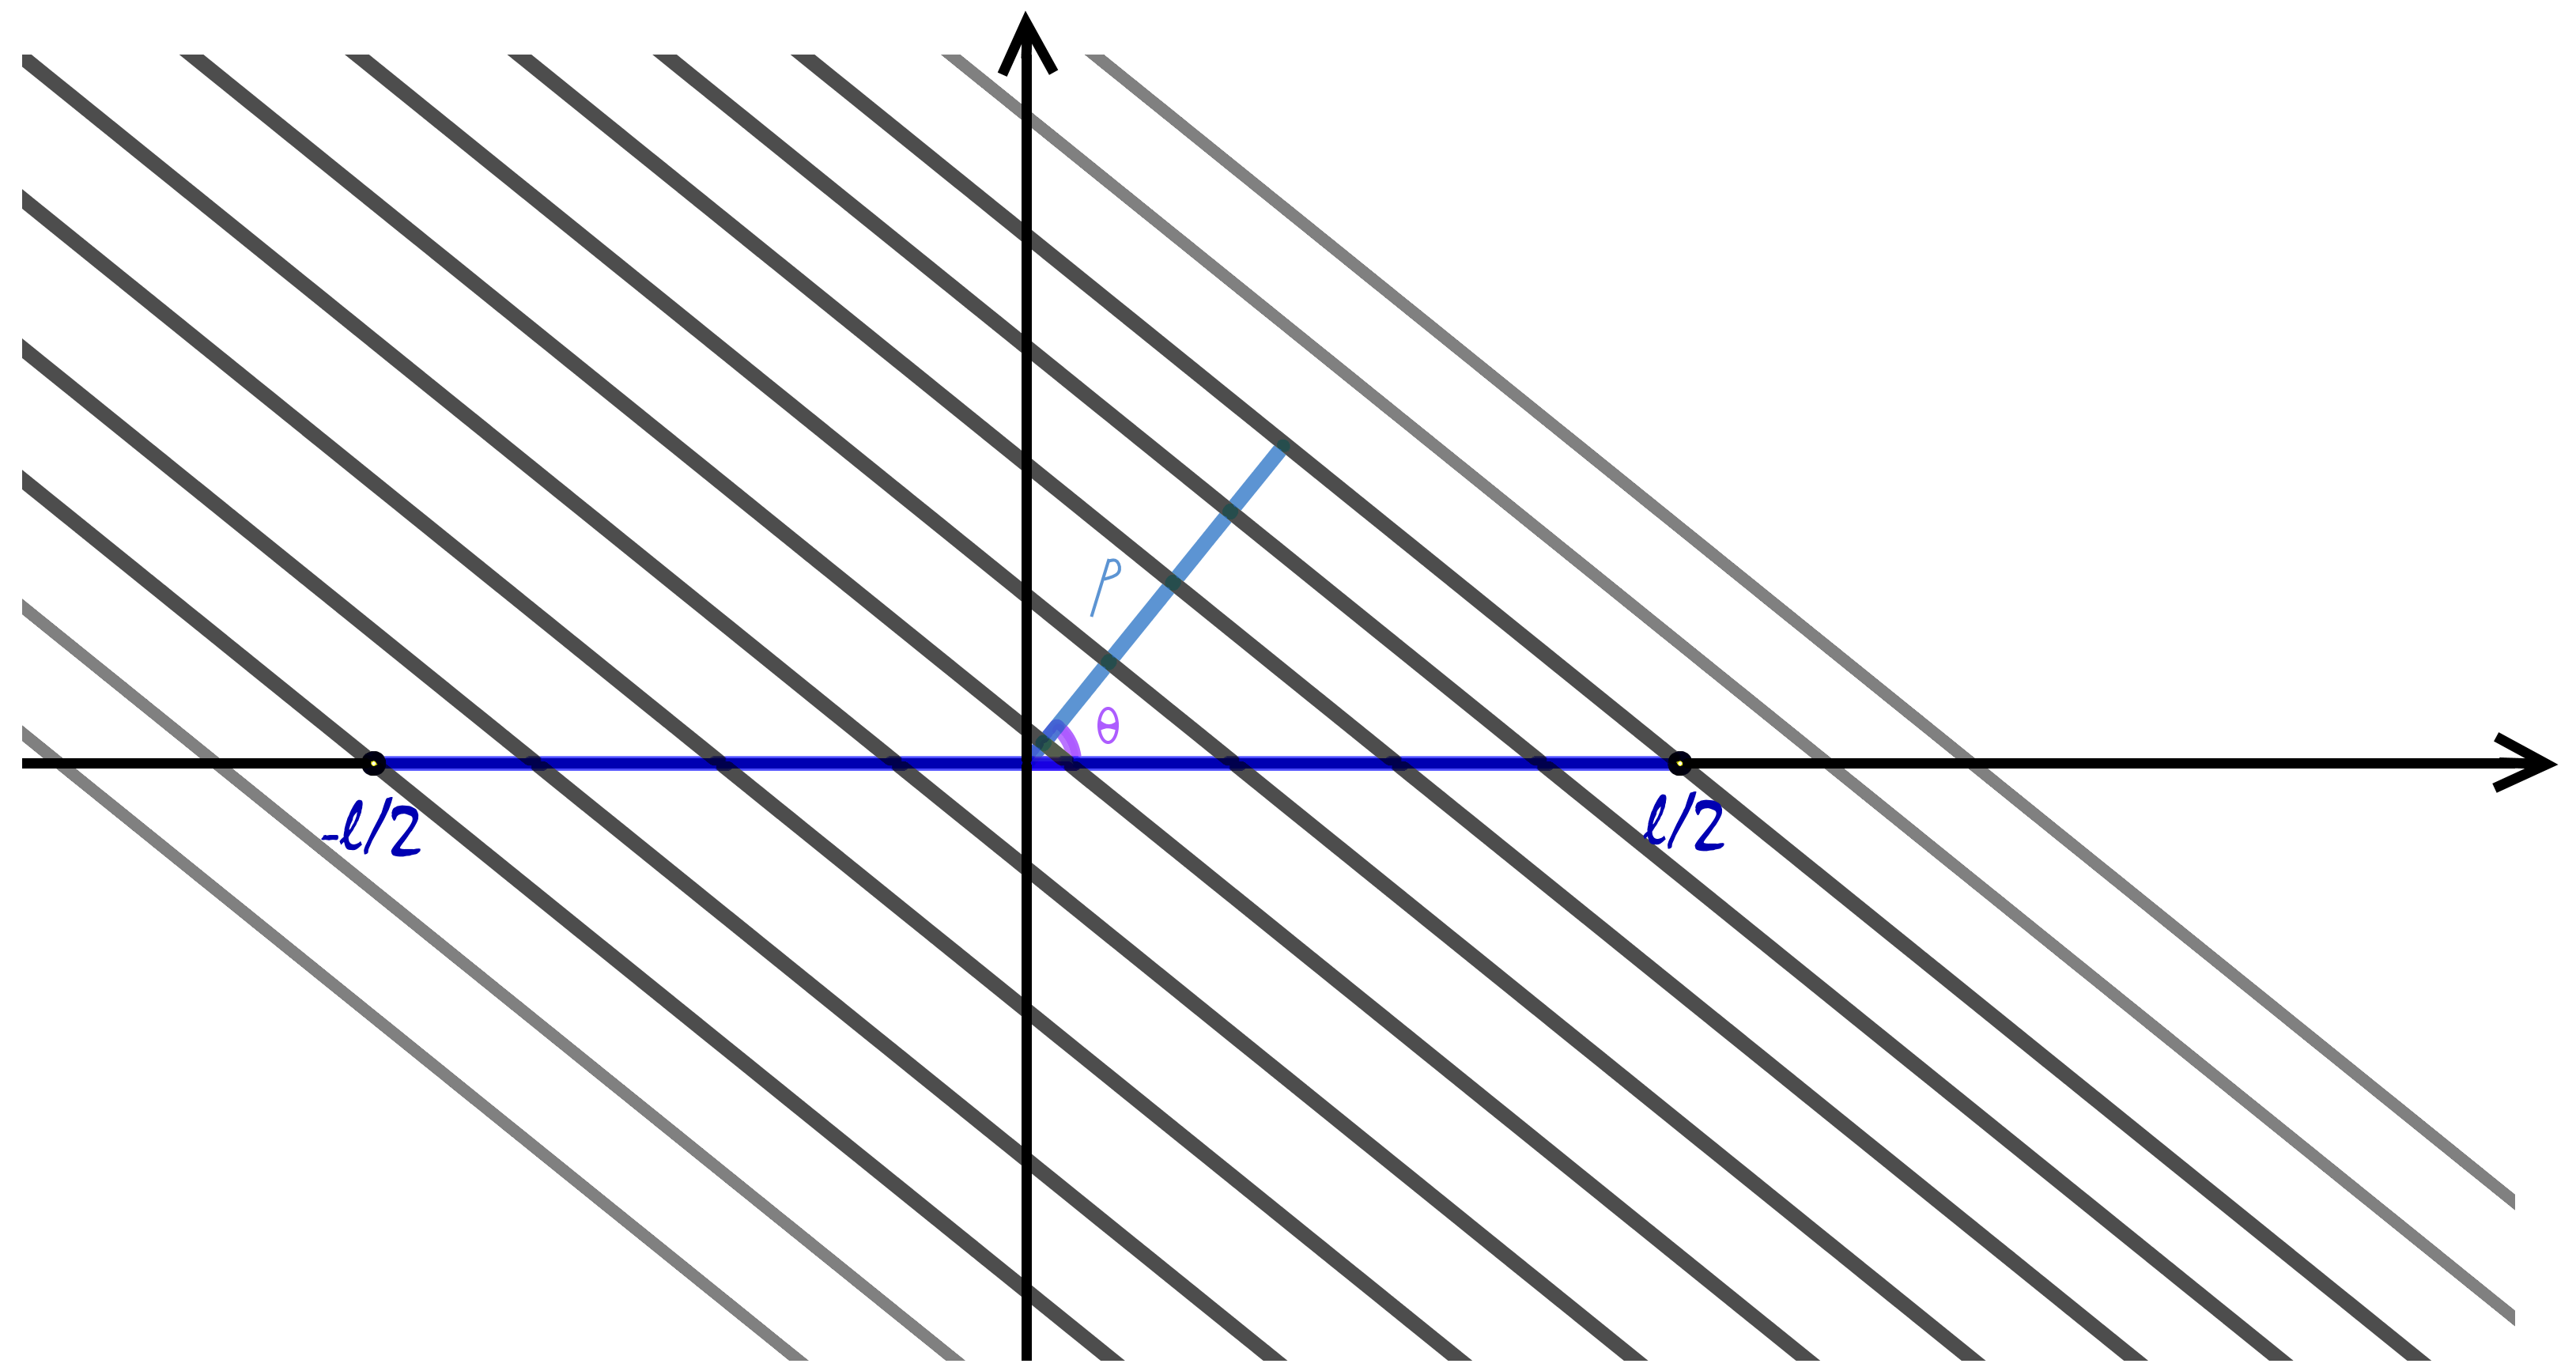
\includegraphics[width=330pt]{img/figureSegment.png}
Clearly, we need $|\rho| \leq \frac{l}{2} |\cos (\theta)|$.
This is true for $\forall \ 0 \leq \theta < \pi$, as the ones from $\pi \leq \theta < 2\pi$ are the same as the ones from $0 \leq \theta < \pi$. Thus, the measure of the segment becomes:
\begin{align}
m(S) =& \iint_S \,d\rho\,d\theta \\
=& \int_{0}^{\pi} \int_{-\frac{l}{2} |\cos (\theta)|}^{\frac{l}{2} |\cos (\theta)|}  d\rho d\theta \\
=& 2 * \int_{0}^{\pi} \int_{0}^{\frac{l}{2} |\cos (\theta)|}  d\rho d\theta \\
=& 2 * \int_{0}^{\pi} \frac{l}{2} |\cos (\theta)| d\theta
\end{align}
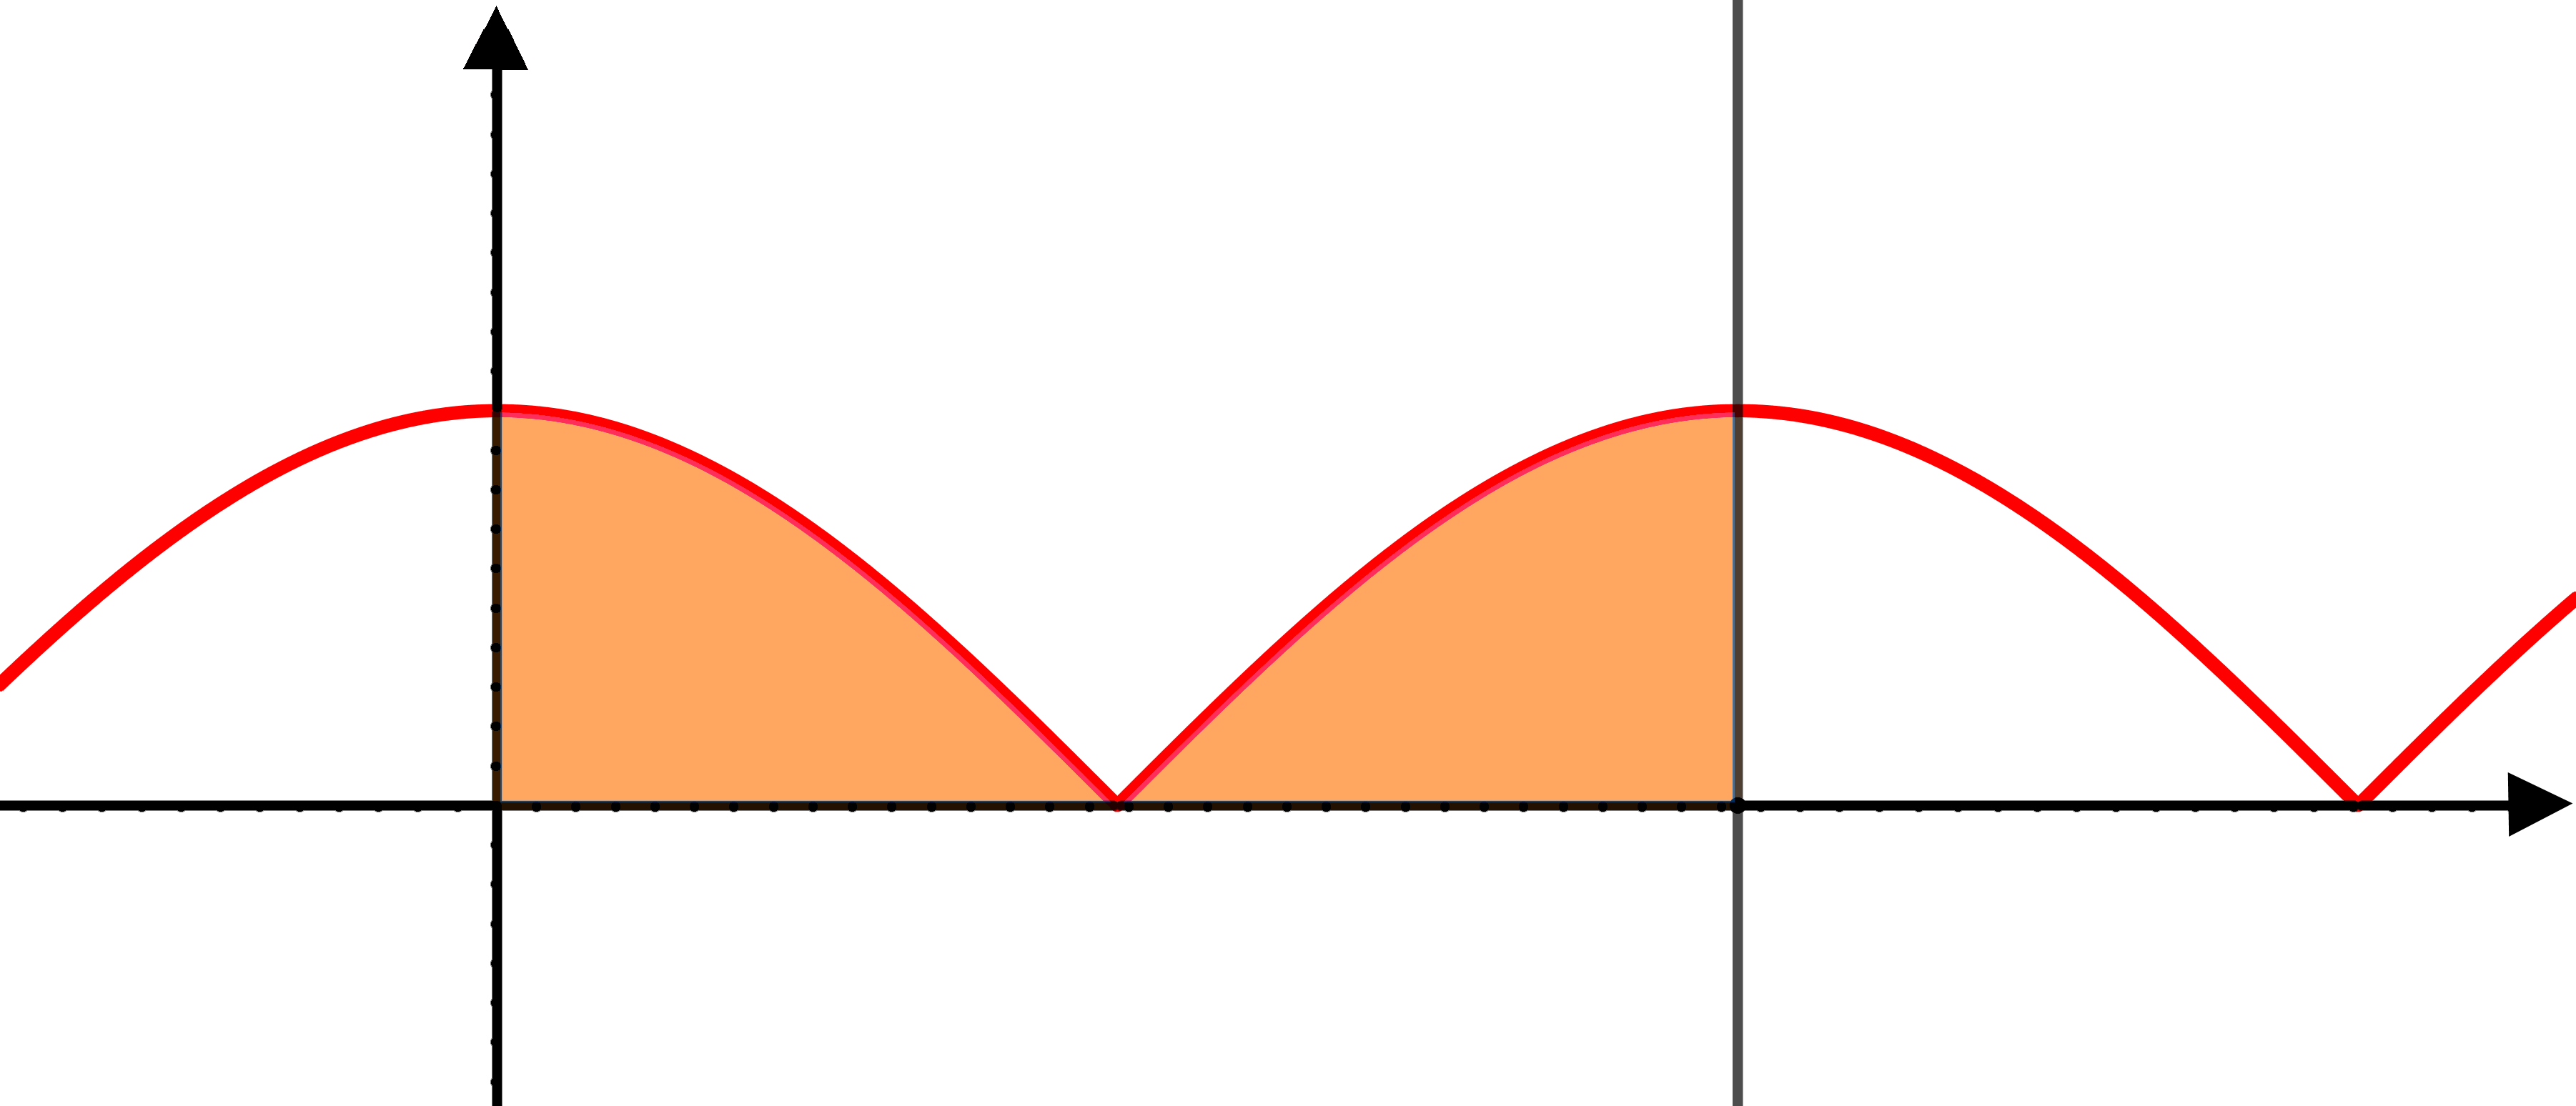
\includegraphics[width=350pt]{img/figureCosIntegral.png}
Here, the red curve is $|\cos(x)|$, the area orange is the area from $0$ to $\pi$ under the curve.
$$ \text{We get:} \int_{0}^{\pi}|\cos (\theta)| d\theta = 2 $$
$$ \text{so}  \int_{0}^{\pi} \frac{l}{2} |\cos (\theta)| d\theta = l$$
$$ \text{thus}  2 * \int_{0}^{\pi} \frac{l}{2} |\cos (\theta)| d\theta = 2* l$$
$$ \text{finally}  m(S) = 2* l \quad \text{( using (11) )}$$

\subsection{More general case: joint segments}
Now, suppose that the curve $C$ is composed of finitely straight segments.
Say that the curve $C$ is composed of $n$ segments $C_i$ of length $l_i \quad (1 \leq i \leq n)$.
So the length of $C$ is $l=\sum_{i=1}^n l_i$.
We have $\forall 1 \leq i \leq n, m(C_i)=l_i$.
Also, $m(C) = \sum_{i=1}^n  m(C_i)$
Thus $m(C) = \sum_{i=1}^n  m(C_i) = \sum_{i=1}^n  l_i = l$

\subsection{General case: a curve}
Finally, let $C$ be a regular curve of length $l$, parameterized by $\gamma(t): [a,b] \to \mathbb{R}^2$
Let $n \in \mathbb{N}$. Now, let $x_i = a + i *(\frac{b-a}{n}) \quad \forall \ 0 \leq i \leq n$.
Then as C is smooth, if $n$ is large enough, the part of curve $\gamma(t): [x_i, x_{i+1}] \to \mathbb{R}^2$ become straight lines.
Thus, we can use the previous calculations to get that:
Thus $m(C) = l$



\section{Applications}
\subsection{Length of a circle}
Take a circle $C$ of radius $r$.
We need to measure the set of lines that crosses the circle, counted with multiplicity:

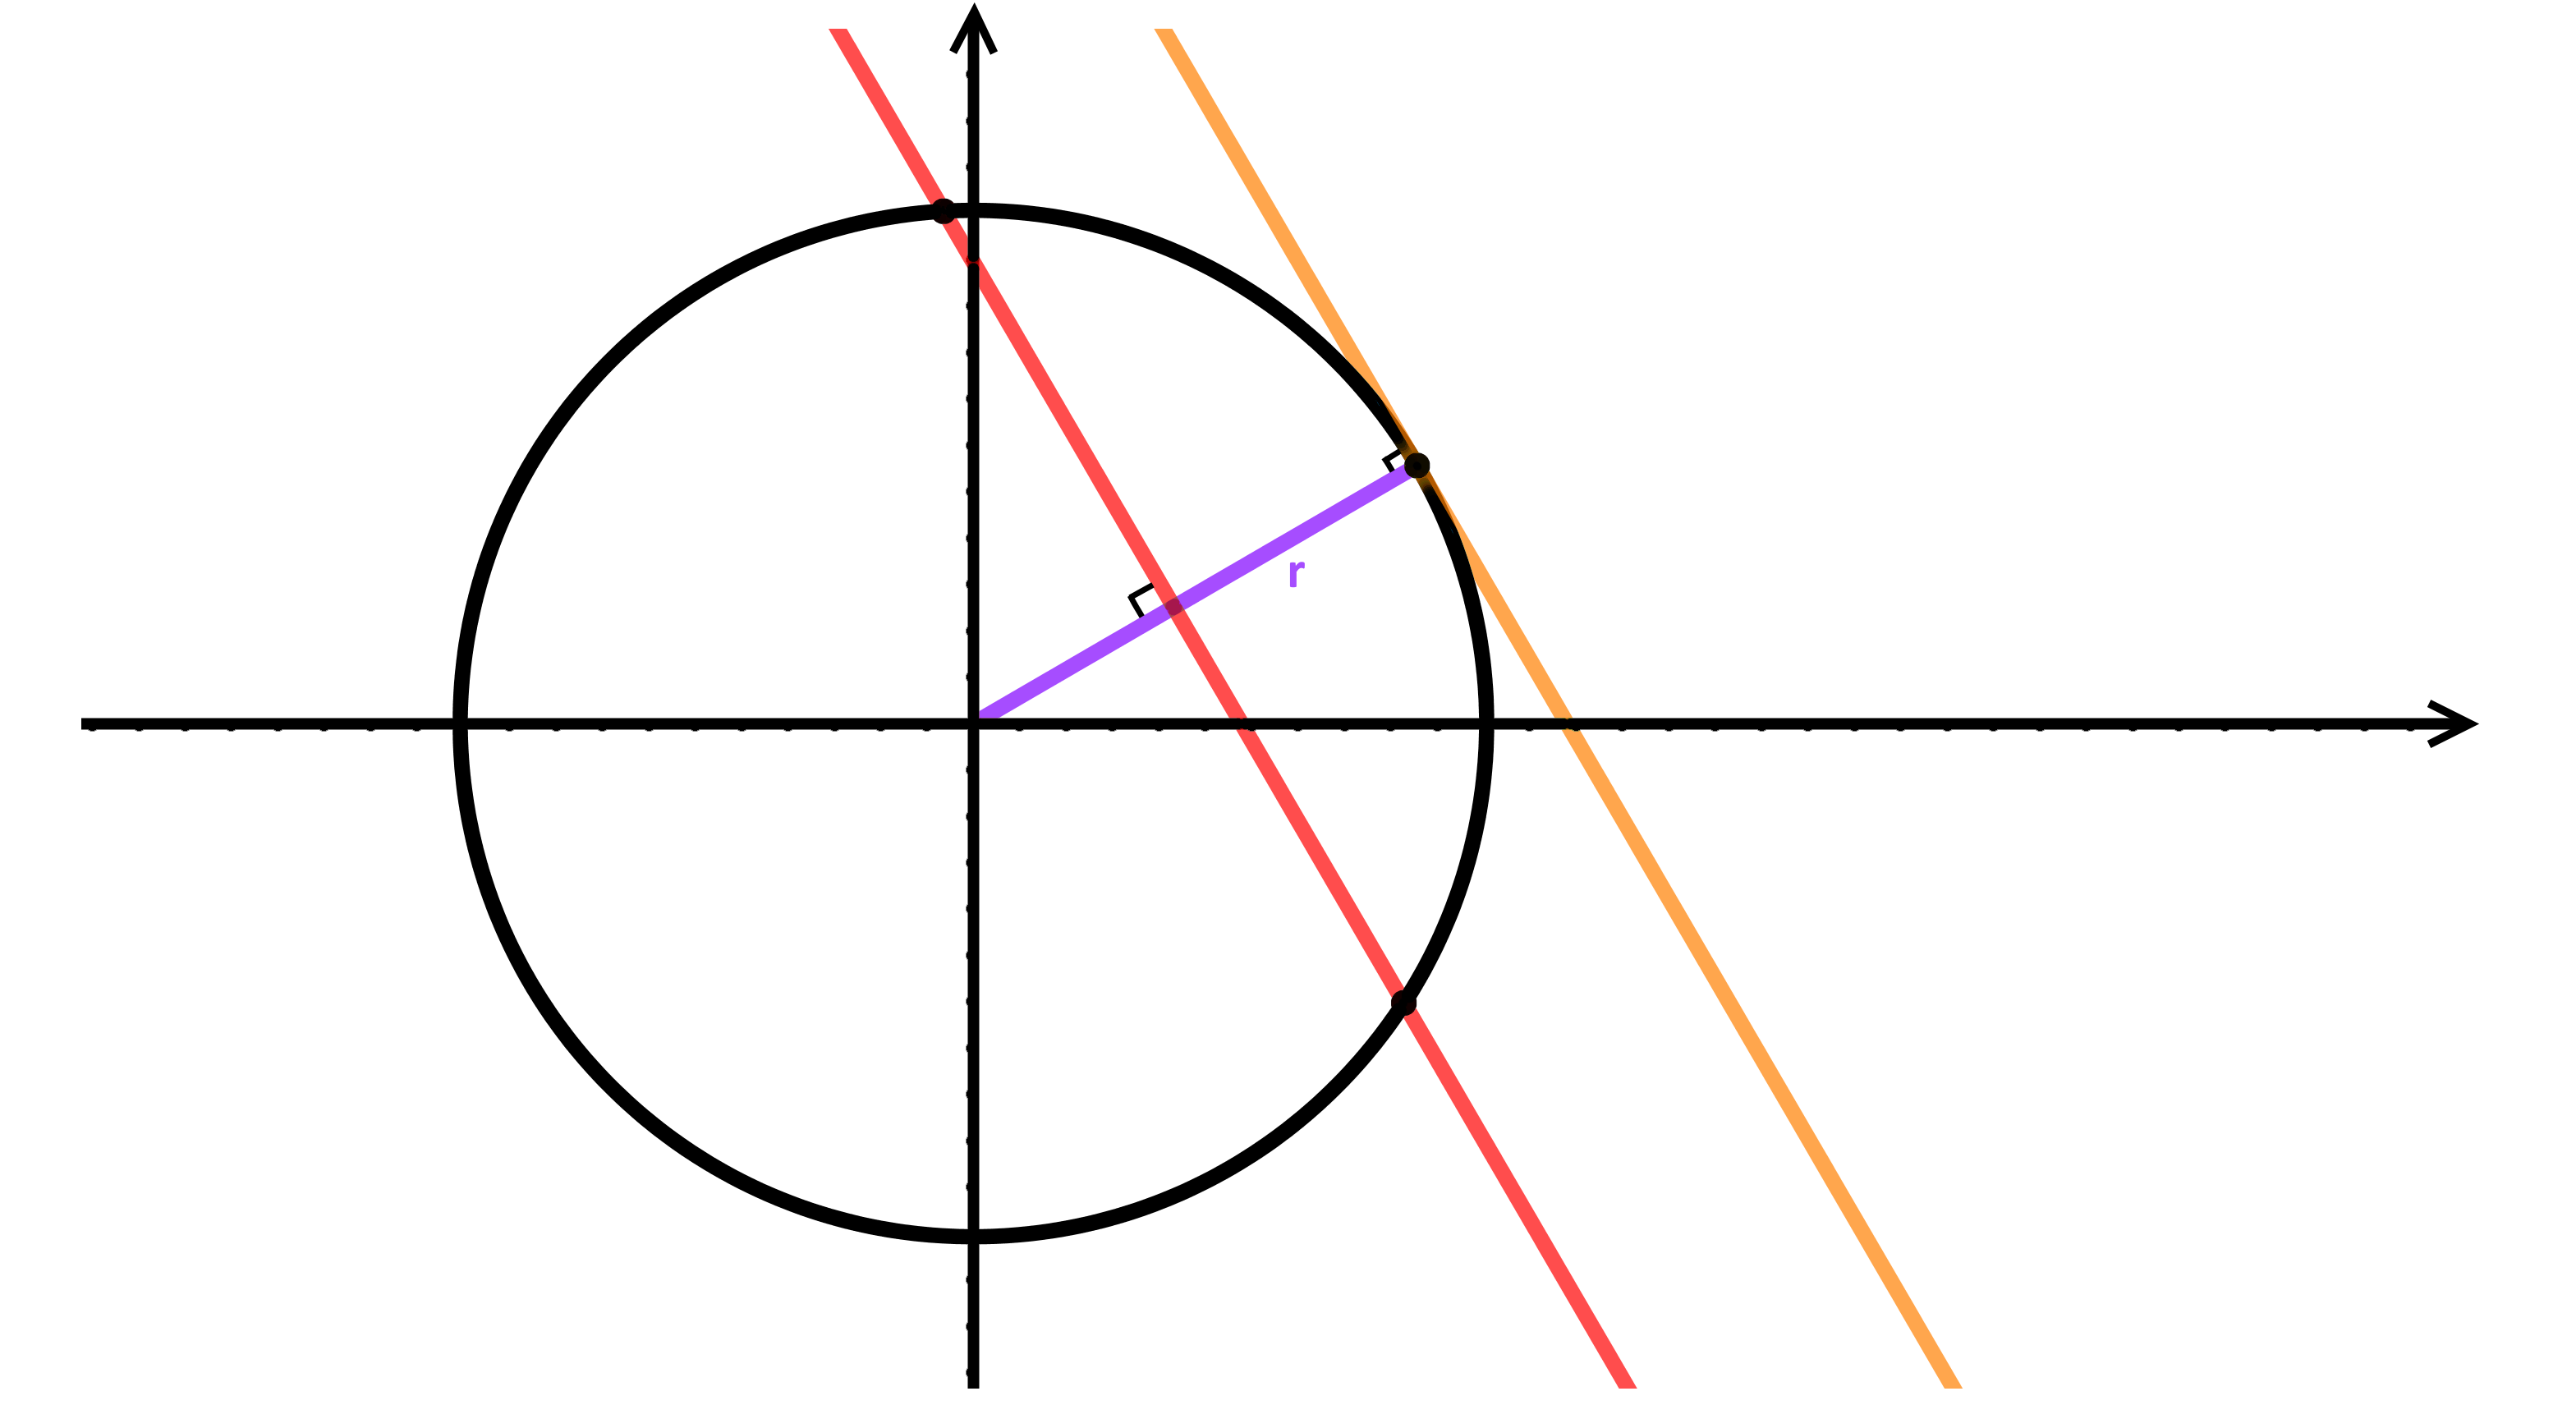
\includegraphics[width=350pt]{img/figureCircleExample.png}
Here, we get that $\forall 0 \leq \theta \leq 2\pi$, the line represented by $(\rho, \theta)$ is crossing the circle once if $\rho = r$, twice if $\rho < r$ and none if $\rho > r$.
So let $f:\mathbb{R} \to \mathbb{R}$ be such that:
$$f(x) = \left\{
\begin{array}{r c l}
2 \quad if \ x < r\\
1 \quad if \ x = r\\
0 \quad if \ x > r
\end{array}
\right.$$
Thus, the measure of the set of lines crossing $C$ counted with multiplicity is:
\begin{align}
m(C) =& \int_0^{2\pi}\int_0^{+\infty} f(x) dx\,d\theta \\
=& \int_0^{2\pi}\int_0^{r} 2 \ dx\,d\theta \\
=& \int_0^{2\pi} 2 r \ d\theta \\
=& \ 4 \pi r = 2* 2\pi r
\end{align}
And we already know that this is twice the length of the circle of radius $r$.
Therefore, we checked the formula for circles.

\subsection{Physically: DNA}
It is true that this formula doesn't really help for curves like circles, because we know other ways to derive the formula that are much easier, but the power of Cauchy-Crofton's Formula is that it can be applied to nice curves like circles as well as very complicated curves (as long as they are regular). Also, as this formula is "just" an integral, we can make a computer calculate an approximation of it. That's why it is very used in calculating the length of DNA segments: the curve of the DNA may be very messy, be remains regular, and an approximation is usually enough (we do not need the very exact value).






\end{document}
